\documentclass[11pt,a4paper]{article}

% Typography & Page Layout
\usepackage[margin=1in]{geometry}
\usepackage[utf8]{inputenc}
\usepackage[T1]{fontenc}
\usepackage{lmodern}
\usepackage{microtype}
\usepackage{setspace}
\onehalfspacing

% Mathematics
\usepackage{amsmath,amssymb,amsthm,bm}

% Tables & Figures
\usepackage{booktabs}
\usepackage{threeparttable}
\usepackage{graphicx}
\usepackage{tikz}
\usetikzlibrary{arrows.meta,positioning,fit,backgrounds}

% Citations & Hyperlinks
\usepackage[authoryear,round]{natbib}
\usepackage[colorlinks=true,linkcolor=blue!60!black,citecolor=blue!60!black,urlcolor=blue!60!black]{hyperref}

% Title Metadata
\title{\textbf{Isolating the Generative AI Labor Shock from Monetary Tightening:} \\
\large A Multivariate Conditional Forecasting Comparison of Bayesian VARs, Deep Learning, and Zero-Shot Foundation Models}

\author{
  Eda Kal Ar{\i}ca\thanks{Department of Statistics, Middle East Technical University (METU), Ankara, T{\"u}rkiye.}
  \and
  Esra {\c{S}}ekerci\footnotemark[1]
}

\date{\today}

\begin{document}

\maketitle

\begin{abstract}
\noindent
The public release of generative artificial intelligence (AI) in late 2022 coincided directly with the Federal Reserve's monetary tightening cycle, creating a major econometric identification problem in separating technological labor displacement from policy-induced cooling. Standard intervention dummies cannot disentangle simultaneous macroeconomic disturbances that propagate through credit markets and real activity with distinct lags. Using a tightly coupled six-variable monthly U.S. macro-financial system from FRED-MD spanning 2010--2026, we ask whether systematic post-2022 conditional forecast errors in total nonfarm payrolls (\texttt{PAYEMS}) and job openings (\texttt{HWI}) reveal an exogenous structural break attributable to generative AI once realized monetary policy (\texttt{FEDFUNDS}), broad liquidity (\texttt{M2SL}), and corporate credit spreads (\texttt{BAA10YM}) are held fixed. We benchmark classical econometric specifications---an unrestricted BIC-selected VAR($p$) and a Minnesota-prior Bayesian VAR with Cholesky-identified impulse response functions and Waggoner--Zha conditional forecasts---against modern learning-based architectures, namely a Temporal Fusion Transformer / LSTM trained with known future policy covariates and zero-shot time-series foundation models (Chronos and TimesFM). Preliminary empirical diagnostics reveal a pronounced post-2022 decoupling: between October 2022 and August 2026, \texttt{PAYEMS} expanded by $+3.3\%$ while \texttt{HWI} contracted by $-32.2\%$, accompanied by a collapse in stationary vacancy--payroll correlation from $r = +0.41$ pre-2022 to $r = -0.10$ post-2022.

\vspace{0.6em}
\noindent\textbf{Keywords:} Bayesian VAR; Conditional Forecasting; Generative AI; Labor Market Vacancies; Monetary Policy Transmission; Time-Series Foundation Models.\\
\textbf{JEL Classification:} C32, C53, E52, J23, O33.
\end{abstract}

\section{Introduction}
\label{sec:intro}

Evaluating the aggregate labor-market impact of generative artificial intelligence (AI) poses a classic macroeconomic identification challenge. The widespread public adoption of generative AI following November 2022 overlapped directly with the sharpest Federal Reserve monetary tightening cycle in four decades. Consequently, any slowdown in U.S. hiring observed since late 2022 reflects an unknown combination of endogenous policy-induced cooling and potential exogenous technological labor displacement.

Simple structural-break dummy regressions are ill-suited for this environment because monetary tightening transmits sequentially through financial conditions, corporate credit spreads, and industrial output before reaching vacancies and aggregate employment. Instead, a \emph{multivariate conditional forecasting} design \citep{waggoner1999conditional,banbura2015conditional,crump2021large} enables us to estimate historical macro-financial transmission dynamics strictly on pre-generative-AI data and then project counterfactual labor-market paths conditional on the realized post-2022 trajectories of monetary policy and financial stress. Systematic forecast shortfalls that persist after conditioning on realized policy paths provide direct empirical evidence of an unmodeled structural shift.

This paper addresses two linked questions:
\begin{quote}
\emph{Does the systematic forecast error in U.S. employment (\texttt{PAYEMS}) and job openings (\texttt{HWI}) post-2022 reveal a structural break attributable to the generative AI shock, and how do classical Bayesian VARs compare to modern deep learning and zero-shot foundation models in isolating this effect?}
\end{quote}

We make three contributions. First, we model aggregate employment (\texttt{PAYEMS}) jointly with job openings (\texttt{HWI}) inside a six-variable macro-financial system, capturing the institutional reality that firms freeze vacancies well before reducing net payroll headcount \citep{pater2017beveridge}. Second, we systematically compare parametric Bayesian shrinkage models against non-linear neural sequence models with known future covariates \citep{lim2021temporal} and zero-shot foundation models \citep{ansari2024chronos,das2024decoder} on an identical pre-/post-2022 evaluation split. Third, we propose explicit identification and robustness diagnostics---including COVID-19 outlier scaling \citep{lenza2022estimate}, ordering sensitivity, and pre-AI placebo break tests---to guard against spurious break detection.

The remainder of the paper is organized as follows. Section~\ref{sec:lit} reviews the related literature. Section~\ref{sec:data} describes the FRED-MD dataset, transmission structure, and exploratory regime shifts. Section~\ref{sec:methodology} formalizes the classical and learning-based models. Section~\ref{sec:results} presents the empirical evaluation design and results, Section~\ref{sec:robustness} outlines robustness analyses, and Section~\ref{sec:conclusion} concludes.

\section{Literature Review}
\label{sec:lit}

Our study bridges three strands of econometric and machine learning research.

\paragraph{Bayesian VARs and Conditional Macroeconomic Forecasting.}
Vector autoregressions with Bayesian shrinkage have become the workhorse framework for multivariate macroeconomic forecasting and scenario analysis. \citet{waggoner1999conditional} established the exact posterior sampling algorithm for conditional forecasts in dynamic multivariate models, which \citet{banbura2015conditional} and \citet{crump2021large} extended to large cross-sections of U.S. macroeconomic and financial series. Prior hyperparameter selection via marginal likelihood maximization \citep{giannone2015prior} and post-pandemic evaluations \citep{sznajderska2023bayesian,korobilis2025exploring} show that well-regularized BVARs deliver credible structural impulse responses and competitive density forecasts even across turbulent regimes. Moreover, \citet{lenza2022estimate} demonstrate that explicitly accommodating COVID-19 innovation volatility prevents March--April 2020 outliers from distorting parameter estimates.

\paragraph{Nonlinear Monetary Transmission and Labor Market Dynamics.}
Recent empirical macroeconomics emphasizes that monetary policy and uncertainty shocks propagate nonlinearly across economic regimes. \citet{primiceri2005time} introduced time-varying parameter SVARs with stochastic volatility to capture evolving monetary transmission, while \citet{eksi2022time} document pronounced time variation in how uncertainty and financial frictions affect U.S. unemployment. Similarly, \citet{caldara2023macroeconomic} highlight dynamic feedback between real activity, corporate credit spreads, and macro-financial volatility, and \citet{debortoli2023asymmetric} document sign- and state-dependent asymmetries in monetary policy tradeoffs. On the labor side, \citet{pater2017beveridge} demonstrates that jointly modeling job vacancies and labor-market stocks is essential for separating aggregate demand shifts from structural matching shocks.

\paragraph{Deep Learning and Zero-Shot Time-Series Foundation Models.}
In parallel, sequence deep learning architectures such as the Temporal Fusion Transformer (TFT) \citep{lim2021temporal} allow non-linear multi-horizon forecasting while explicitly ingesting known future covariates---providing a direct deep-learning analogue to conditional VAR forecasting. More recently, pretrained foundation models such as Chronos \citep{ansari2024chronos} and TimesFM \citep{das2024decoder} have demonstrated strong zero-shot forecasting accuracy across diverse domains without task-specific parameter estimation. Whether these architectures filter macro-financial noise more effectively than parametric shrinkage BVARs when isolating post-2022 structural breaks remains an open empirical question.

\section{Data and Empirical Preliminaries}
\label{sec:data}

We extract $k = 6$ monthly U.S. macroeconomic and financial series from the Federal Reserve Bank of St. Louis FRED-MD database \citep{mccracken2016fredmd}: Industrial Production (\texttt{INDPRO}), Total Nonfarm Payrolls (\texttt{PAYEMS}), the Help-Wanted Index (\texttt{HWI}) as a vacancy proxy, the Effective Federal Funds Rate (\texttt{FEDFUNDS}), M2 Money Stock (\texttt{M2SL}), and the Moody's Seasoned Baa corporate yield spread over 10-Year Treasuries (\texttt{BAA10YM}, constructed directly as $\texttt{BAA} - \texttt{GS10}$).

\begin{table}[htbp]
\centering
\begin{threeparttable}
\caption{FRED-MD Macroeconomic and Financial Series Specification and Summary Statistics (January 2010--September 2026)}
\label{tab:data_summary}
\small
\begin{tabular}{@{}llllrrrr@{}}
\toprule
Series & Description & Role & \texttt{tcode} & Mean & SD & Pre-AI & Post-AI \\
\midrule
\texttt{INDPRO}   & Industrial Production (2017 = 100)       & Real Activity & 5 ($\Delta \ln x_t$)   & 99.44      & 3.38     & 98.94      & 101.05 \\
\texttt{PAYEMS}   & Total Nonfarm Payrolls (thousands)       & Labor Target  & 5 ($\Delta \ln x_t$)   & 145,453.9  & 9,167.8  & 141,780.1  & 157,491.3 \\
\texttt{HWI}      & Help-Wanted Index (job openings)         & Labor Target  & 2 ($\Delta x_t$)       & 6,433.7    & 2,300.3  & 5,969.9    & 7,986.5 \\
\texttt{FEDFUNDS} & Effective Federal Funds Rate (\% p.a.)   & Conditioning  & 2 ($\Delta x_t$)       & 1.52       & 1.83     & 0.59       & 4.54 \\
\texttt{M2SL}     & M2 Money Stock (billions USD)            & Conditioning  & 6 ($\Delta^2 \ln x_t$) & 15,443.4   & 4,846.6  & 13,561.4   & 21,609.9 \\
\texttt{BAA10YM}  & Baa Corporate--10Y Treasury (\% p.a.)    & Conditioning  & 1 ($x_t$)              & 2.33       & 0.54     & 2.52       & 1.72 \\
\bottomrule
\end{tabular}
\begin{tablenotes}[flushleft]
\footnotesize
\item \textit{Notes:} Source is FRED-MD \citep{mccracken2016fredmd}. The full local sample covers January 2010--September 2026 ($T = 201$); the Pre-AI training window spans January 2010--October 2022 ($T_{\text{train}} = 154$) and the Post-AI evaluation window spans November 2022--September 2026 ($T_{\text{test}} = 47$). \texttt{BAA10YM} is constructed as $\texttt{BAA} - \texttt{GS10}$. \texttt{HWI} has one trailing missing observation in September 2026 ($n = 200$). Transformation codes follow \citet{mccracken2016fredmd}.
\end{tablenotes}
\end{threeparttable}
\end{table}


Table~\ref{tab:data_summary} reports full-sample and regime-specific summary statistics across the pre-AI training window (January 2010--October 2022, $T_{\text{train}} = 154$) and the post-2022 evaluation window (November 2022--September 2026, $T_{\text{test}} = 47$; target $T_{\text{test}} = 48$ upon the October 2026 vintage release). Figure~\ref{fig:transmission} summarizes the hypothesized macro-financial transmission channel and our conditional identification structure.

\begin{figure}[htbp]
\centering
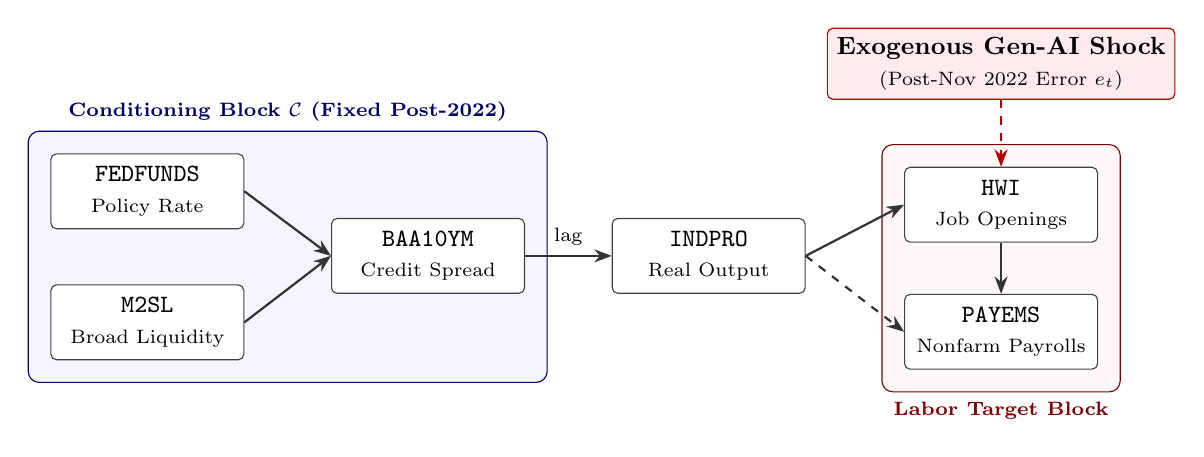
\begin{tikzpicture}[
  node distance=0.85cm and 1.15cm,
  box/.style={rectangle, draw=black!75, rounded corners=2pt, align=center, minimum width=2.45cm, minimum height=0.95cm, font=\small, fill=white},
  shock/.style={rectangle, draw=red!70!black, fill=red!8, rounded corners=2pt, align=center, minimum width=3.4cm, minimum height=0.85cm, font=\small\bfseries},
  arr/.style={-{Stealth[length=2.2mm]}, thick, draw=black!80},
  sarr/.style={-{Stealth[length=2.2mm]}, thick, dashed, draw=red!70!black}
]
  \node[box] (ff) {\texttt{FEDFUNDS}\\{\scriptsize Policy Rate}};
  \node[box, below=0.7cm of ff] (m2) {\texttt{M2SL}\\{\scriptsize Broad Liquidity}};
  \node[box, right=1.1cm of ff, yshift=-0.82cm] (spread) {\texttt{BAA10YM}\\{\scriptsize Credit Spread}};
  \node[box, right=1.1cm of spread] (ip) {\texttt{INDPRO}\\{\scriptsize Real Output}};
  \node[box, right=1.25cm of ip, yshift=0.65cm] (hwi) {\texttt{HWI}\\{\scriptsize Job Openings}};
  \node[box, below=0.65cm of hwi] (pay) {\texttt{PAYEMS}\\{\scriptsize Nonfarm Payrolls}};
  \node[shock, above=0.85cm of hwi] (ai) {Exogenous Gen-AI Shock\\{\scriptsize\normalfont (Post-Nov 2022 Error $e_t$)}};

  \begin{scope}[on background layer]
    \node[draw=blue!40!black, fill=blue!4, rounded corners=4pt, inner sep=8pt, fit=(ff)(m2)(spread), label={[font=\scriptsize\bfseries, text=blue!40!black]above:Conditioning Block $\mathcal{C}$ (Fixed Post-2022)}] {};
    \node[draw=red!50!black, fill=red!3, rounded corners=4pt, inner sep=8pt, fit=(hwi)(pay), label={[font=\scriptsize\bfseries, text=red!50!black]below:Labor Target Block}] {};
  \end{scope}

  \draw[arr] (ff.east) -- (spread.west);
  \draw[arr] (m2.east) -- (spread.west);
  \draw[arr] (spread.east) -- node[above, font=\scriptsize]{lag} (ip.west);
  \draw[arr] (ip.east) -- (hwi.west);
  \draw[arr, dashed] (ip.east) -- (pay.west);
  \draw[arr] (hwi.south) -- (pay.north);
  \draw[sarr] (ai.south) -- (hwi.north);
\end{tikzpicture}
\caption{Macro-financial transmission mechanism and conditional forecasting identification scheme.}
\label{fig:transmission}
\end{figure}

Exploratory diagnostics on the stationary FRED-MD transformations reveal a striking post-2022 structural shift. During the pre-AI training sample (2010--2022), monthly changes in job openings (\texttt{HWI}) correlate positively with both payroll growth ($r = +0.412$) and industrial production growth ($r = +0.413$), while \texttt{INDPRO} and \texttt{PAYEMS} co-move strongly ($r = +0.870$). Over the post-2022 tightening window, however, \texttt{HWI} decouples sharply from payroll growth ($r = -0.103$), output growth ($r = -0.048$), and contemporaneous changes in \texttt{FEDFUNDS} ($r = +0.008$). In levels, total nonfarm payrolls expanded by $+3.3\%$ between October 2022 and August 2026 (153.9M to 159.0M) while job openings declined by $-32.2\%$ (10,447 to 7,079), motivating formal conditional counterfactual testing.

\section{Econometric and Learning-Based Methodology}
\label{sec:methodology}

Let $\mathbf{y}_t = (\texttt{FEDFUNDS}_t,\, \texttt{M2SL}_t,\, \texttt{BAA10YM}_t,\, \texttt{INDPRO}_t,\, \texttt{HWI}_t,\, \texttt{PAYEMS}_t)^\top \in \mathbb{R}^6$ denote the multivariate vector observed at monthly frequency. All trainable models are estimated strictly on $t \in \{1,\dots,T_{\text{train}}\}$ (January 2010--October 2022).

\subsection{Classical Econometric Models}

\paragraph{Unrestricted VAR($p$).}
As a stationary linear baseline, we estimate a reduced-form VAR($p$) on FRED-MD transformed series:
\begin{equation}
  \mathbf{y}_t = \mathbf{c} + \sum_{\ell=1}^{p} \mathbf{A}_\ell \mathbf{y}_{t-\ell} + \boldsymbol{\varepsilon}_t,
  \qquad \boldsymbol{\varepsilon}_t \sim \mathcal{N}(\mathbf{0}, \boldsymbol{\Sigma}),
  \label{eq:var}
\end{equation}
selecting lag order $p$ via the Bayesian Information Criterion (BIC).

\paragraph{Bayesian VAR with Minnesota Priors and Conditional Forecasting.}
To address over-parameterization and preserve rich lag dynamics, we estimate a Bayesian VAR with conjugate Normal--Inverse-Wishart Minnesota shrinkage priors \citep{giannone2015prior}. Structural monetary transmission is validated via Cholesky-identified impulse response functions ($\boldsymbol{\Sigma} = \mathbf{P}\mathbf{P}^\top$). Following \citet{waggoner1999conditional} and \citet{banbura2015conditional}, we partition the system into the conditioning policy/financial block $\mathcal{C} = \{\texttt{FEDFUNDS}, \texttt{M2SL}, \texttt{BAA10YM}\}$ and target labor series $i \in \{\texttt{PAYEMS}, \texttt{HWI}\}$, fix $\mathbf{y}^{\mathcal{C}}_{T_{\text{train}}+1:T_{\text{train}}+H}$ at its realized post-2022 path, and compute conditional forecast errors:
\begin{equation}
  e_{i,\, T_{\text{train}}+h} = y_{i,\, T_{\text{train}}+h} - \hat{y}_{i,\, T_{\text{train}}+h \mid T_{\text{train}},\, \mathbf{y}^{\mathcal{C}}_{T_{\text{train}}+1:T_{\text{train}}+h}},
  \qquad h = 1,\dots,T_{\text{test}}.
  \label{eq:cond_err}
\end{equation}
Persistent negative realizations of $e_{i,T_{\text{train}}+h}$ lying outside posterior credible intervals represent systematic labor-market shortfalls unexplained by realized monetary tightening.

\subsection{Learning-Based Models}

\paragraph{Temporal Fusion Transformer (TFT) / LSTM.}
We train a deep sequence model \citep{lim2021temporal} strictly on pre-2022 multivariate data, supplying $\mathbf{y}^{\mathcal{C}}$ as known future covariates over the post-2022 horizon. Hyperparameters (hidden state size, number of layers, learning rate, and dropout) are selected via expanding-window time-series cross-validation to prevent look-ahead leakage.

\paragraph{Zero-Shot Foundation Model.}
We evaluate pretrained foundation models---Chronos \citep{ansari2024chronos} and/or TimesFM \citep{das2024decoder}---prompted zero-shot with the pre-2022 historical context. Comparing zero-shot quantile trajectories against the conditional BVAR and trained neural baseline tests whether large-scale pretrained temporal representations adapt more robustly across structural breaks without rigid parametric assumptions.

\begin{table}[htbp]
\centering
\caption{Summary of Candidate Model Specifications}
\label{tab:models}
\small
\begin{tabular}{@{}llll@{}}
\toprule
Model & Family & Post-2022 Conditioning & Identification / Tuning \\
\midrule
Unrestricted VAR($p$) & Classical & Unconditional & BIC lag order selection \\
Bayesian VAR (BVAR) & Classical & Waggoner--Zha ($\mathcal{C}$ fixed) & Minnesota prior; Cholesky IRFs \\
TFT / LSTM & Deep Learning & Known future covariates ($\mathcal{C}$) & Expanding-window time-series CV \\
Chronos / TimesFM & Foundation & Pre-2022 context only & Zero-shot pretrained inference \\
\bottomrule
\end{tabular}
\end{table}

\section{Empirical Results}
\label{sec:results}

\subsection{Falsifiable Hypotheses}
Prior to model estimation, we state three testable predictions:
\begin{enumerate}
  \item \textbf{Monetary explanation of payrolls (\texttt{PAYEMS}):} The conditional BVAR explains the majority of post-2022 deceleration in aggregate employment strictly via monetary tightening.
  \item \textbf{Unexplained vacancy break (\texttt{HWI}):} Job openings exhibit a statistically significant negative conditional forecast error ($e_{\texttt{HWI},t} < 0$), reflecting a targeted hiring freeze associated with generative AI adoption.
  \item \textbf{Non-linear model advantage:} Deep learning and foundation models isolate the vacancy--payroll divergence more robustly than the linear BVAR.
\end{enumerate}

\subsection{Unit-Root, Cointegration, and IRF Validation}
\textit{[To be populated following Step~1 ADF/KPSS/Johansen pre-testing and Step~2 Cholesky IRF estimation.]}

\subsection{Conditional Counterfactual Trajectories and Break Tests}
\textit{[To be populated with BVAR posterior conditional bands, TFT/LSTM counterfactuals, and Newey--West HAC break tests on $e_{\texttt{HWI},t}$ and $e_{\texttt{PAYEMS},t}$.]}

\subsection{Cross-Model Forecast Accuracy Comparison}
Out-of-sample predictive accuracy will be compared using RMSE, MAE, Continuous Ranked Probability Score (CRPS), and \citet{diebold1995comparing} equal predictive accuracy tests (Table~\ref{tab:results_ledger}).

\begin{table}[htbp]
\centering
\caption{Post-2022 Out-of-Sample Evaluation Ledger (Pending Estimation)}
\label{tab:results_ledger}
\small
\begin{tabular}{@{}lrrrrrr@{}}
\toprule
Model & \multicolumn{2}{c}{RMSE} & \multicolumn{2}{c}{CRPS} & \multicolumn{2}{c}{Mean Error ($\bar{e}_i$)} \\
\cmidrule(lr){2-3}\cmidrule(lr){4-5}\cmidrule(lr){6-7}
 & \texttt{PAYEMS} & \texttt{HWI} & \texttt{PAYEMS} & \texttt{HWI} & \texttt{PAYEMS} & \texttt{HWI} \\
\midrule
Unrestricted VAR($p$) & --- & --- & --- & --- & --- & --- \\
Bayesian VAR (Conditional) & --- & --- & --- & --- & --- & --- \\
TFT / LSTM (Covariates) & --- & --- & --- & --- & --- & --- \\
Chronos / TimesFM (Zero-Shot) & --- & --- & --- & --- & --- & --- \\
\bottomrule
\end{tabular}
\end{table}

\section{Robustness Checks}
\label{sec:robustness}

To verify that identified post-2022 forecast errors are not artifacts of econometric specification, we will conduct four robustness checks: (i) explicit COVID-19 innovation-volatility scaling following \citet{lenza2022estimate}; (ii) alternative Cholesky variable orderings; (iii) a pre-AI placebo conditional break test evaluated over 2017--2019; and (iv) sensitivity to Minnesota prior tightness and lag order.

\section{Conclusion}
\label{sec:conclusion}

\textit{[To be completed upon completion of empirical estimation and robustness analyses.]}

\bibliographystyle{apalike}
\bibliography{references}

\end{document}
